\documentclass{beamer}

\usepackage[utf8]{inputenc}
\usepackage{svg}
\usepackage{graphicx}
\usepackage{lmodern}

\usetheme{AnnArbor}
\usecolortheme{beaver}

\begin{document}

\title{Bioinformatics of the Immune System}
\author{Lasath Fernando}

\begin{frame}
\titlepage
\end{frame}

\section{Background}
\subsection{Immune Response}
\begin{frame}
  \frametitle{Immunoglobulins}

  \begin{columns}
    \begin{column}{5cm}
    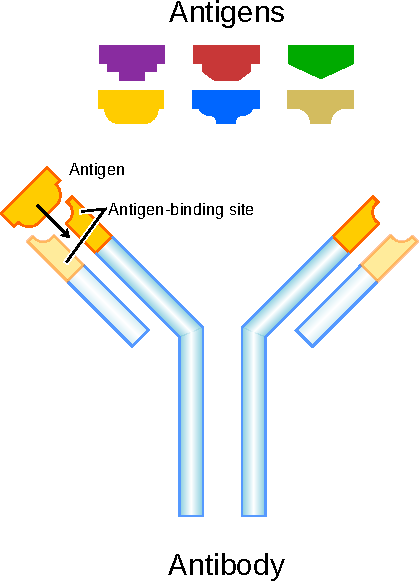
\includegraphics[width=\textwidth]{antibody.pdf}
    \end{column}
    \begin{column}{5cm}
    \begin{itemize}
     \item Also known as antibodies
     \item Y-shaped protein
     \item Binds to a very specific antigen, which is doomed from that point.
     \item Needs to be extremely specific as a result.
     \item Produced by B-Cells
    \end{itemize}

    \end{column}
  \end{columns}

\end{frame}

\begin{frame}
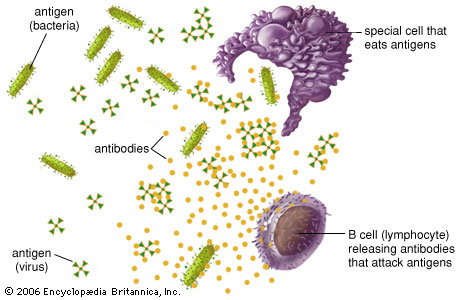
\includegraphics[width=\textwidth]{antigens-antibodies.jpg}
\end{frame}

\begin{frame}
\frametitle{B-Cell}
\begin{columns}
  \begin{column}{.5\textwidth} 
    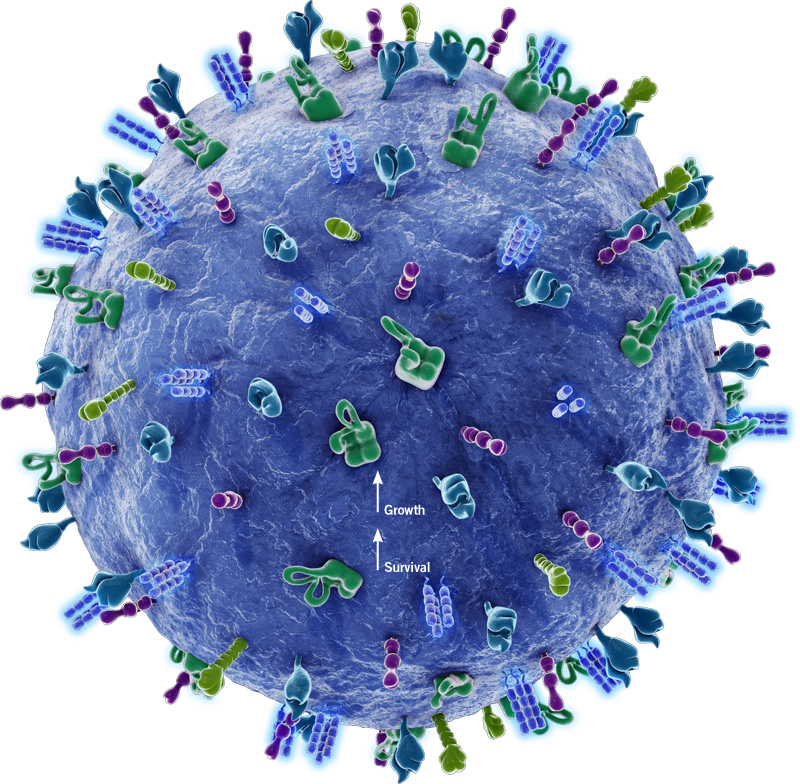
\includegraphics[width=\textwidth]{b-cell.jpg}
  \end{column}
  \begin{column}{.5\textwidth} 
    \begin{itemize}
     \item Produces a particular antibody
     \item Some of them detach and float around on their own
     \item Contains the rearranged (mutated) DNA
    \end{itemize}
  \end{column}
\end{columns}
\end{frame}

\subsection{Combination Process}

\begin{frame}
\frametitle{Combination Process}
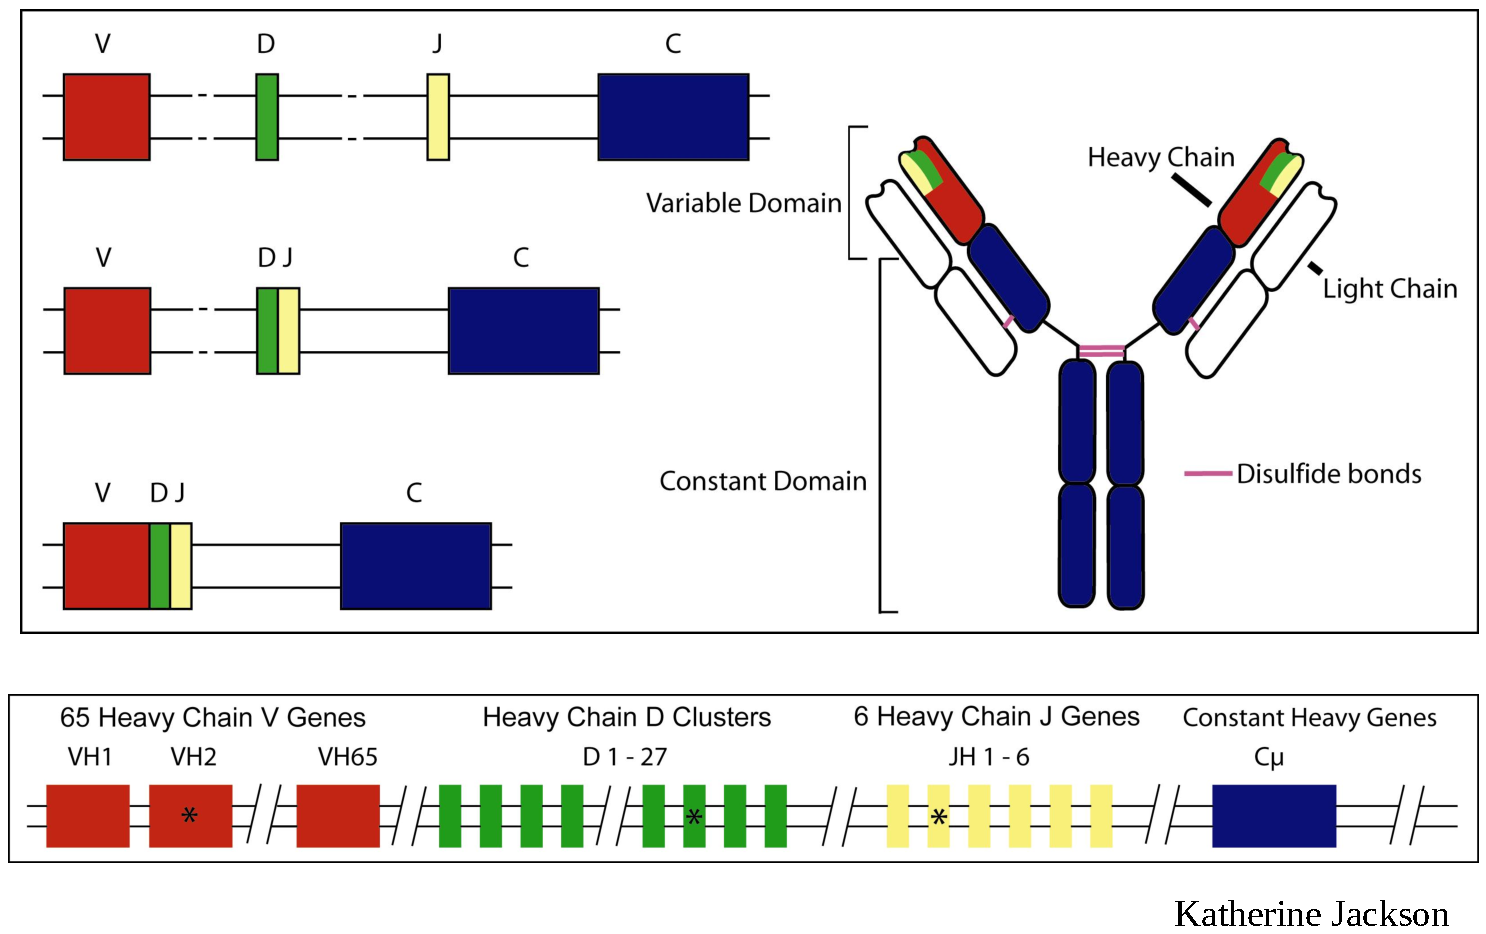
\includegraphics[width=\textwidth]{rearrangement.pdf}
%% Mutiple V,D,J genes per person, 
%% one of each gets picked, and combined
%% they then mutate as well. (non-deterministic process)
\end{frame}

\subsection{Machine Learning}

\begin{frame}
\frametitle{Hidden Markov Model}
\begin{columns}
  \begin{column}{.5\textwidth} 
    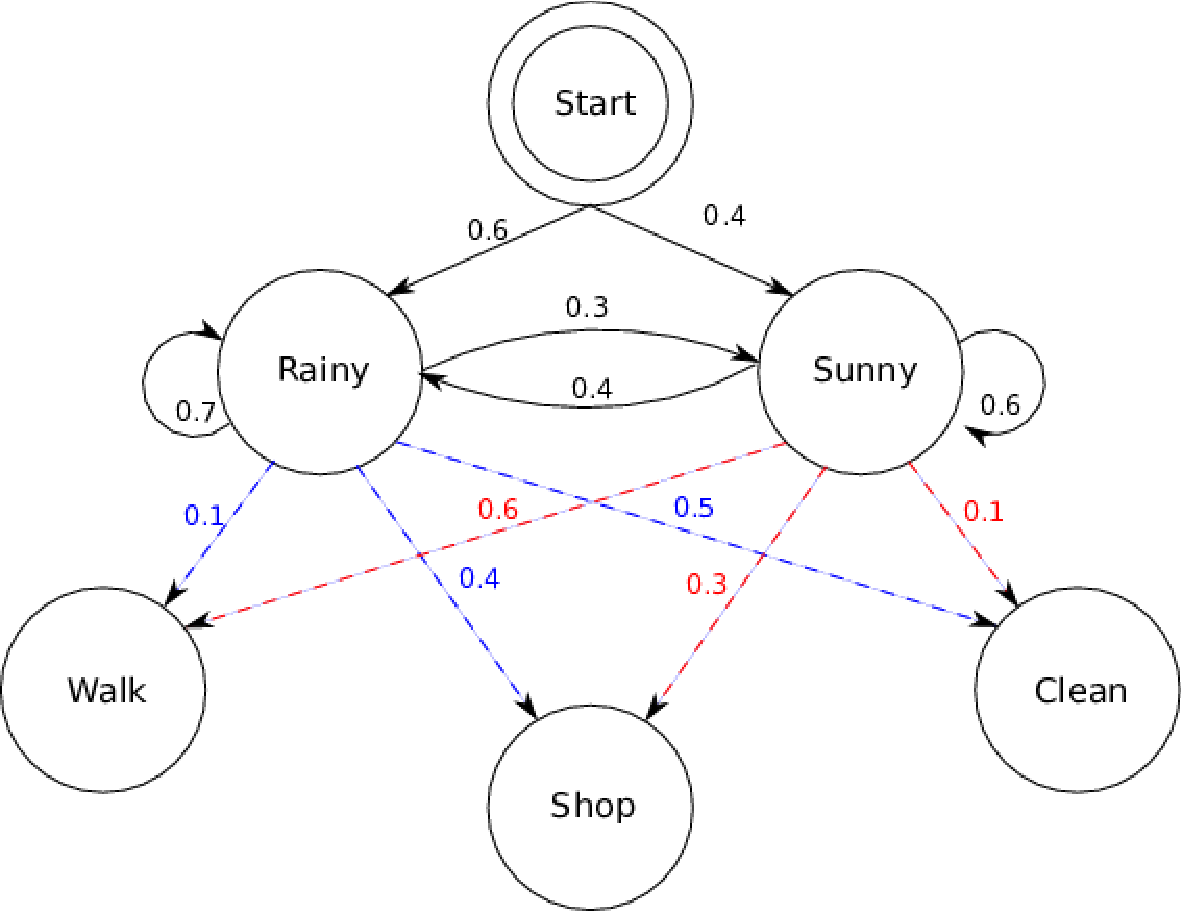
\includegraphics[width=\textwidth]{hmm-graph.pdf}
  \end{column}
  \begin{column}{.5\textwidth} 
    \begin{itemize}
      \item Commonly used in machine learning for speech recognition
      \item Markov Chain where the states can not be observed directly
    \end{itemize}
  \end{column}
\end{columns}
\end{frame}

\section{Motivation}

\subsection{IHMMuneAlign}

\begin{frame}
\frametitle{IHMMuneAlign}
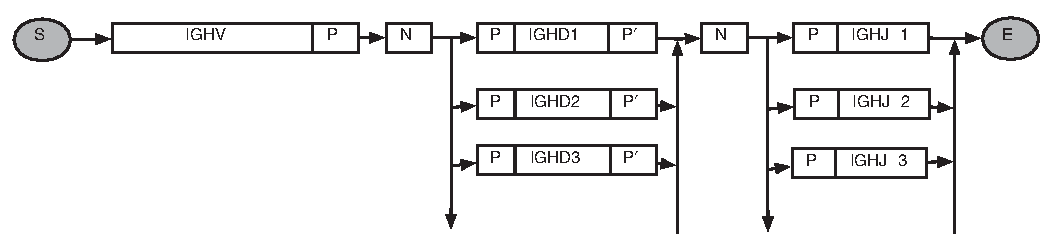
\includegraphics[width=\textwidth]{model.pdf}
\begin{itemize}
 \item Is given the rearranged gene sequence that's found in the B-Cell (For a particular Immunoglobulin).
 \item Attempts to determine the sequences that formed it
 \item Represents the known steps of the recombination process as states in a HMM.
 \item Runs viterbi algorithm to determine the chain of states that caused the observations (The rearranged sequence)
\end{itemize}
\end{frame}

\begin{frame}
\frametitle{Motivation}
 \begin{itemize}
  \item Current gene-sequencing technologies are good at processing lots of small sequences
  \item Not so good with long sequences
  \item Rearranged gene in a B-Cell is easy to find
  \begin{itemize}
   \item Start is marked by constant region
   \item End is marked by a few possible genes
  \end{itemize}
  \item Sequencing technologies are improving - getting up to 100,000 rearranged antibody genes from a single patient
  \item Means IHMMuneAlign \emph{needs to be faster}
 \end{itemize}
\end{frame}

\section{Plan}

\begin{frame}
\frametitle{Existing Implementation}
\begin{itemize}
 \item Written in Java
 \item Uses BioJava
 \item Takes items in FASTA format
 \item Does iteration in launcher script
 \begin{itemize}
  \item Overhead of spinning up/tearing down JVM after each one
  \item Reading data files each time
  \item Invaliding caches/buffers etc
 \end{itemize}
\end{itemize}
\end{frame}

\begin{frame}[fragile]
\frametitle{Initial Run}
\begin{verbatim}
>AJ512650.1| Homo sapiens partial mRNA for immunoglobulin
heavy chain variable region (IGHV gene), clone 43
CTCGAGTCGGGGGGAGGCTGGGTACAGCCTGGCAGGTCCCTGAGACTCTCCTGTTCA
GCCTCTGGACTCACCTTTGATGATTATGCCATGCACTGGGTCCGGCAAGCTCCAGGG
AAGGGCCTGGAGTGGGTCTCCGGTATTAGTTGGAACAGTGGTGTTAGAGCCTATGCG
GACTCTGTGAAGGGCCGATTCACCATCTCCAGAGACAACGGCAAGAATTCCCTGTAT
CTGCAAATGAACAGTCTGAGACCTGAGGACACGGCCTTGTATTATTGTGCAAAAGAT
ATTCGGGCTGCTACCCCATACGCCCTTGATCACTGGGGCCAGGGAGTCCTGGTCACC
GTCTCCTCA
...
\end{verbatim}
\begin{verbatim}
7.42s user 0.24s system 198% cpu 3.865 total
\end{verbatim}
\end{frame}

\begin{frame}
\frametitle{Existing Implementation}
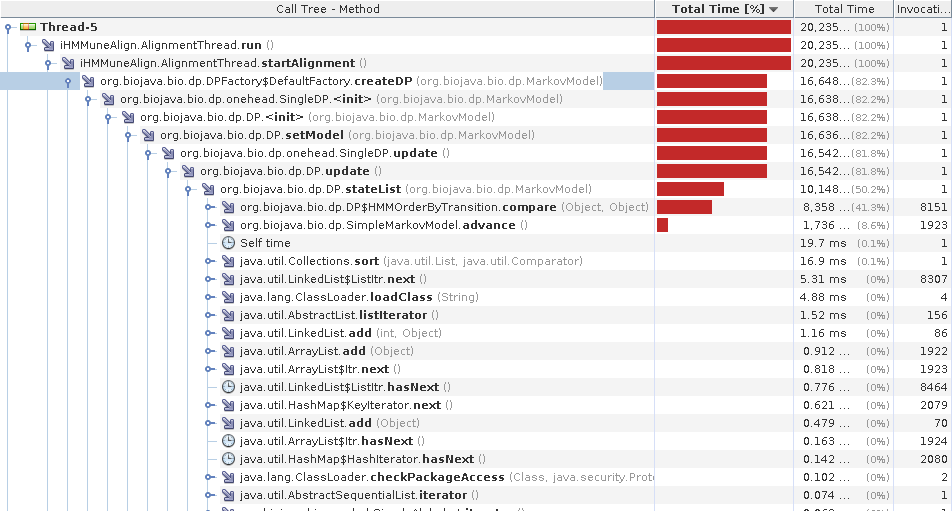
\includegraphics[width=\textwidth]{profile.png}
\end{frame}

\begin{frame}[fragile]
\frametitle{Other Experimentation}
\begin{itemize}
 \item Try different libraries
 \item Modified code to write generated model to file
 \item StochHMM
 \begin{itemize}
  \item General purpose HMM solver
  \item Takes in model in a description file
  \item Crashes, while loading the model
 \end{itemize}
 \item MLPack
 \begin{itemize}
  \item Machine learning library
  \item Too slow
  \item Tries to process entire state space (not sparse)
 \end{itemize}
 \item Custom implementation
 \begin{itemize}
  \item[] \begin{verbatim}0.74s user 0.01s system 99% cpu 0.751 total\end{verbatim}
 \end{itemize}
\end{itemize}
\end{frame}

%% Justify use of C++
%% Justify rewrite 
%% 	binf code

\begin{frame}
\frametitle{Steps From Here}
\begin{itemize}
 \item Based on time
 \item Reimplement model generation part in C++
 \begin{itemize}
  \item Current codebase not extensible
  \item Scalable design
  \item Potentially distributable
  \item High preformance
  \item C++
 \end{itemize}
 \item Fix up HMM (viterbi) implementation
 \item Investigate meaningful ways of sharing computation between runs
 \item Micro-optimize
 \item Investigate improvements to model itself
\end{itemize}

\end{frame}

\end{document}
